% !TEX TS-program = pdflatex
% !TEX encoding = UTF-8 Unicode

% This file is a template using the "beamer" package to create slides for a talk or presentation

\documentclass{beamer}


\mode<presentation>
{
  \usetheme{default}
  % or ...

%  \setbeamercovered{transparent}
  % or whatever (possibly just delete it)
}


\usepackage[english]{babel}

\usepackage[utf8]{inputenc}

\usepackage{graphicx}

\usepackage{times}
\usepackage[T1]{fontenc}
% Or whatever. Note that the encoding and the font should match. If T1
% does not look nice, try deleting the line with the fontenc.
\setbeamertemplate{caption}{\insertcaption}


\title[Building a database on S3] % (optional, use only with long paper titles)
{Presentation of ``Building a database on S3''}

%\subtitle
%{for the seminar in TDT4150 ``Avanserte Databasesystemer''}

\author[Odd M. Trondrud]{Odd M. Trondrud}

\institute[Norwegian University of Technology and Science] 
{
  Presentation of seminar article\\
  TDT4150 ``Avanserte Databasesystemer''\\
  autumn semester of 2013\\
  NTNU
%  No department\\
%  I'm just a student
}

\date[]
{2013-10-22}



% If you have a file called "university-logo-filename.xxx", where xxx
% is a graphic format that can be processed by latex or pdflatex,
% resp., then you can add a logo as follows:

% \pgfdeclareimage[height=0.5cm]{university-logo}{university-logo-filename}
% \logo{\pgfuseimage{university-logo}}



% Delete this, if you do not want the table of contents to pop up at
% the beginning of each subsection:
\AtBeginSubsection[]
{
  \begin{frame}<beamer>{Outline}
    \tableofcontents[currentsection,currentsubsection]
  \end{frame}
}


% If you wish to uncover everything in a step-wise fashion, uncomment
% the following command: 

%\beamerdefaultoverlayspecification{<+->}


\begin{document}

\begin{frame}
  \titlepage
\end{frame}

\begin{frame}{Outline}
  \tableofcontents
  % You might wish to add the option [pausesections]
\end{frame}



\section{Motivation}

\subsection{the assignment was mandatory}

\section{The Article}
  \subsection{What's it about?}
    \begin{frame}{What's it about?}
      \begin{itemize}
      \item
        ``How to build a database on S3''
      \item
        S3 is a utility/cloud storage service
      \item
        Why would you want to do that?
        \begin{itemize}
        \item
          Less infrastructure to maintain
        \item
          \$\$\$ savings?
        \item
          Mad scalability
        \end{itemize}
      \end{itemize}
    \end{frame}

\subsection{The proposed implementation}
  \begin{frame}{The proposed implementation}
  % first image
    \begin{center}
      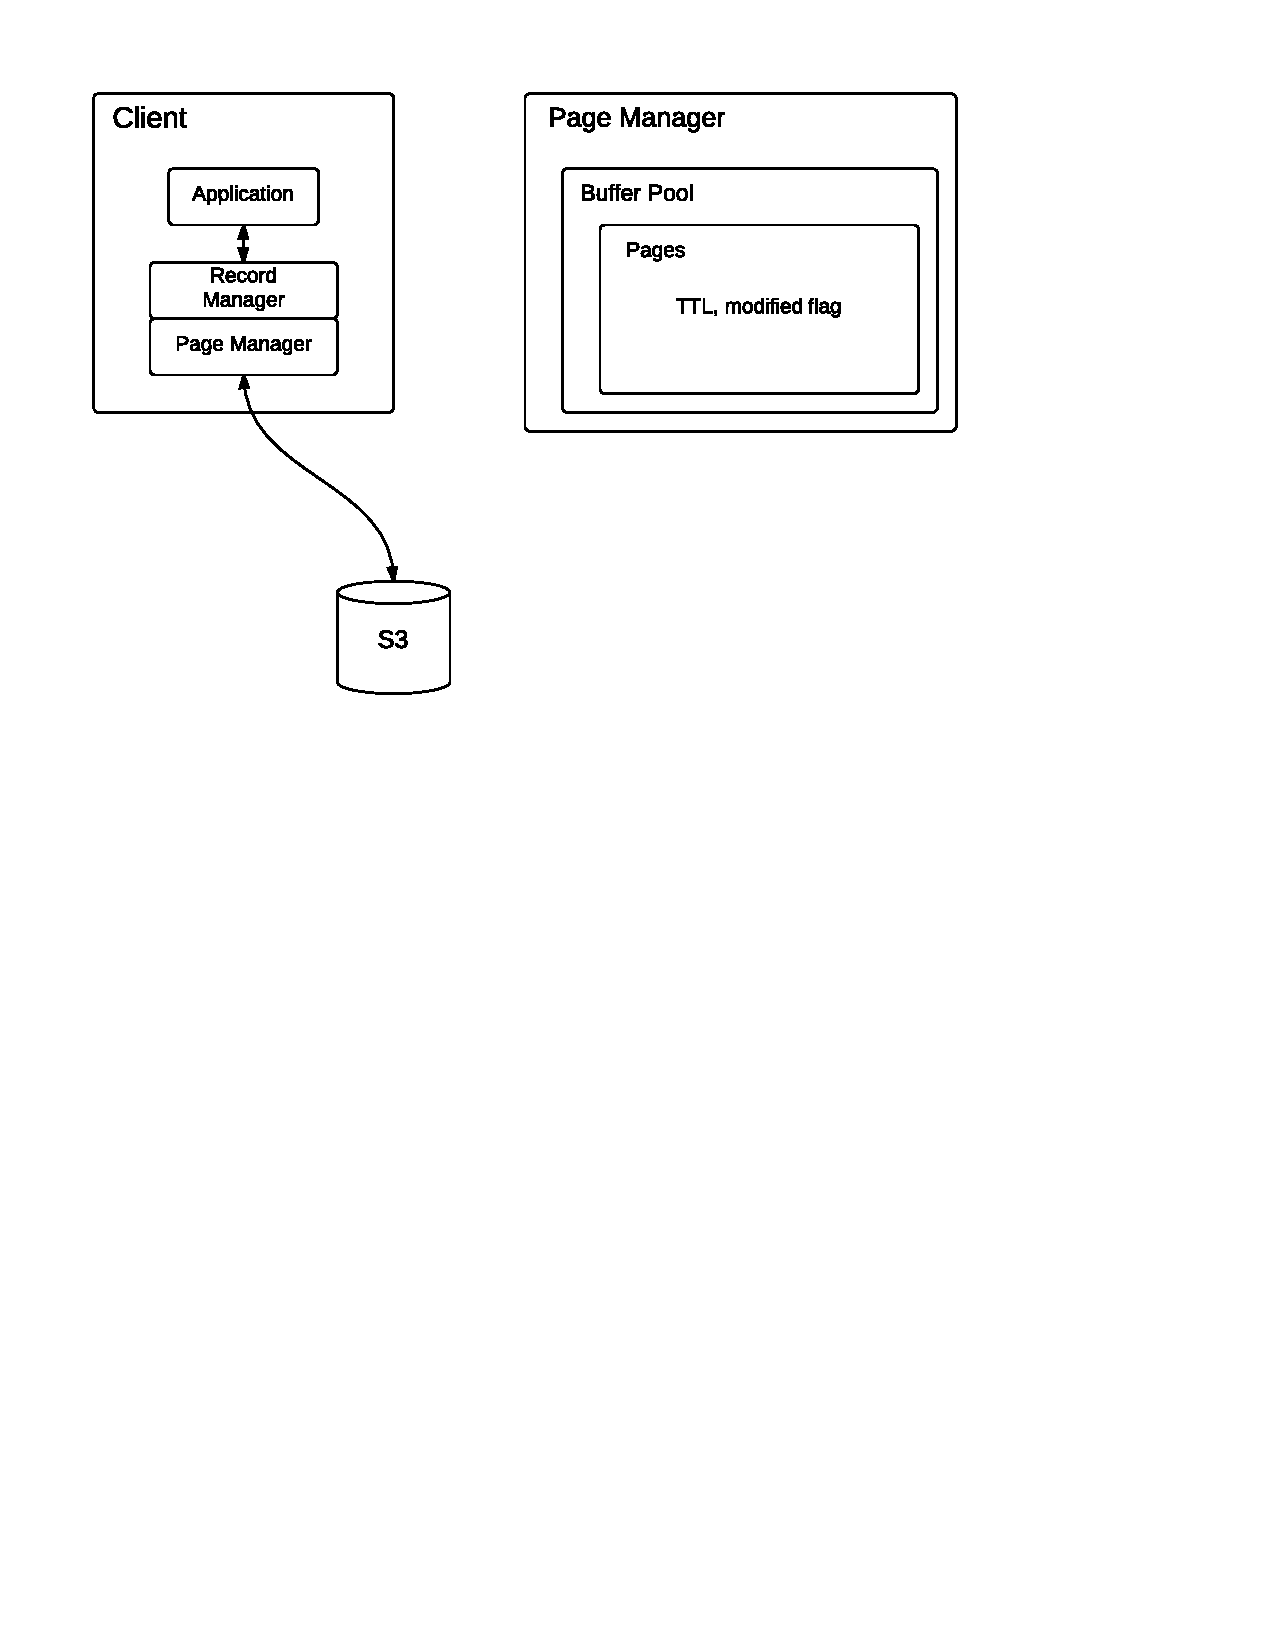
\includegraphics[width=\linewidth]{img/ADB arch 1.pdf}
    \end{center}
  \end{frame}

  \begin{frame}{The proposed implementation}
  % second image
    \begin{center}
      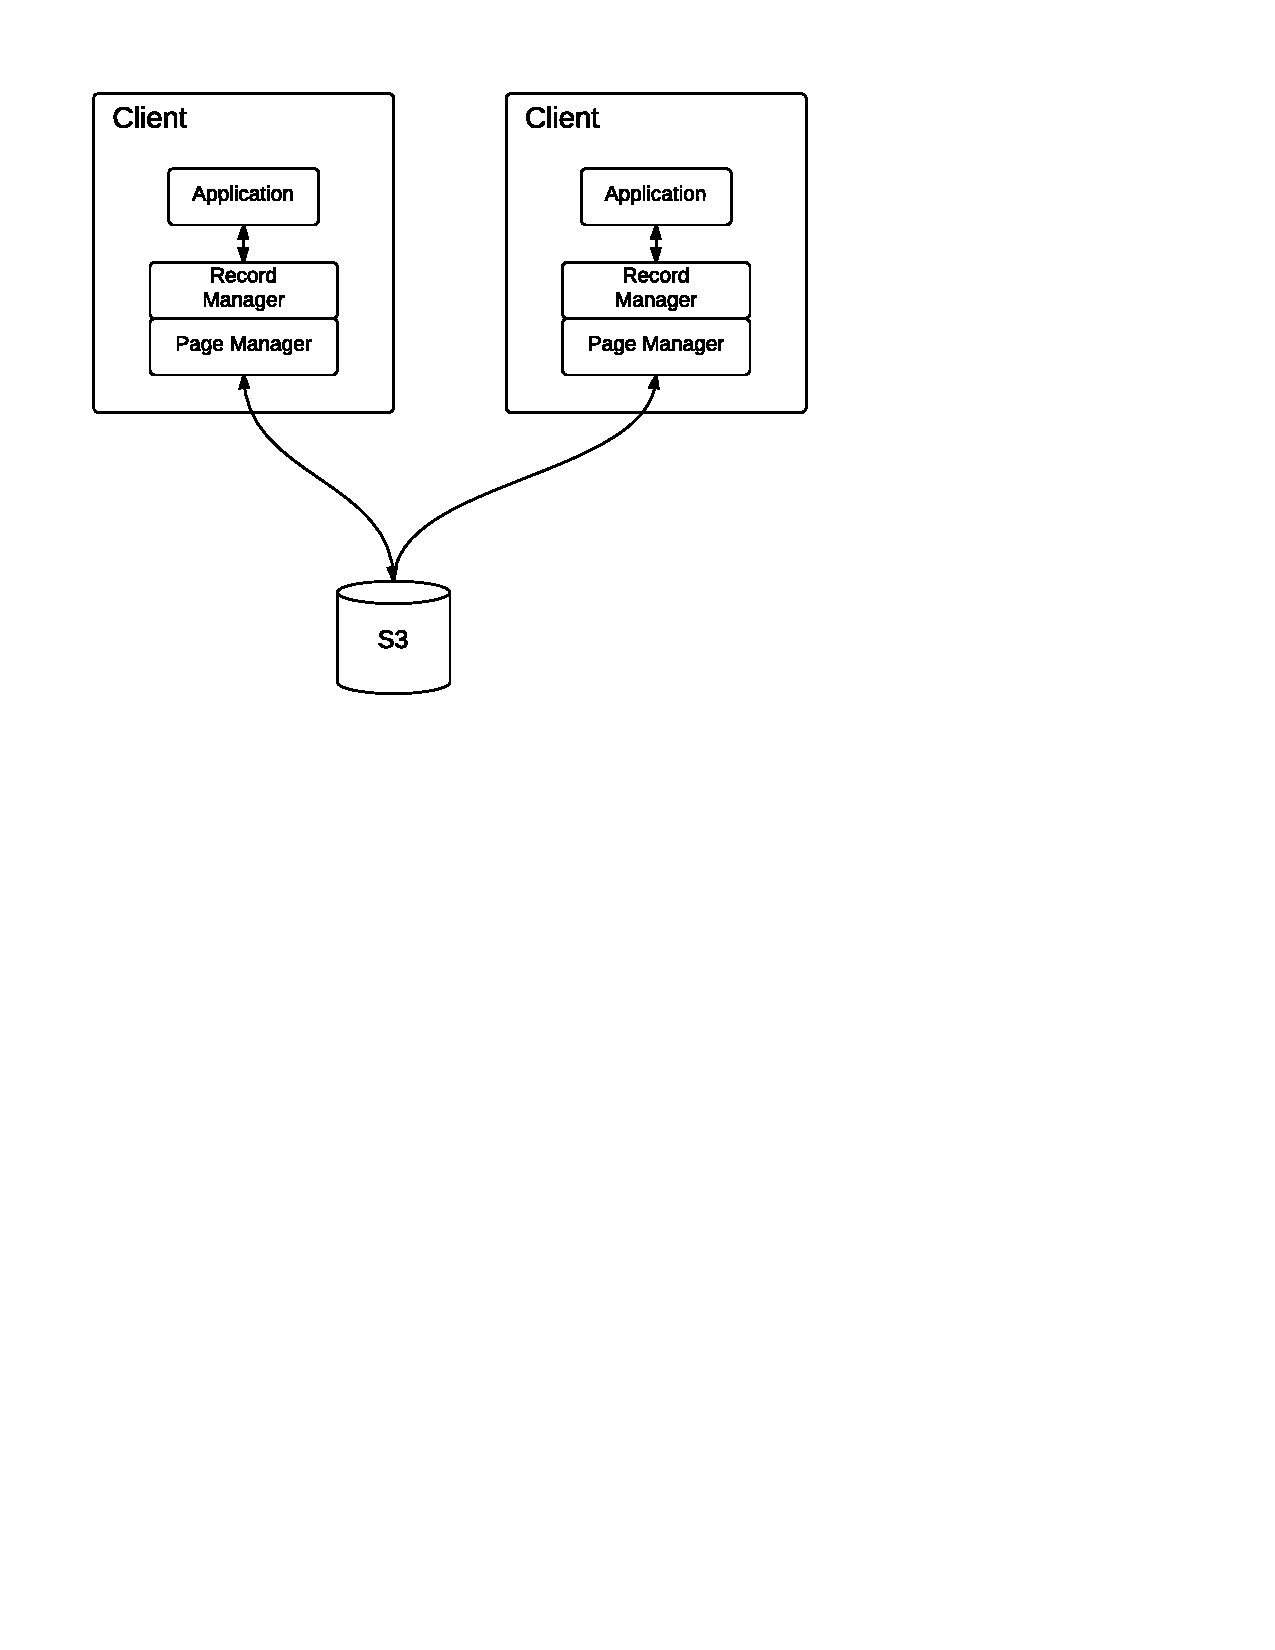
\includegraphics[width=\linewidth]{img/ADB arch 2.pdf}
    \end{center}
  \end{frame}

  \begin{frame}{The proposed implementation}
  % third image
    \begin{center}
      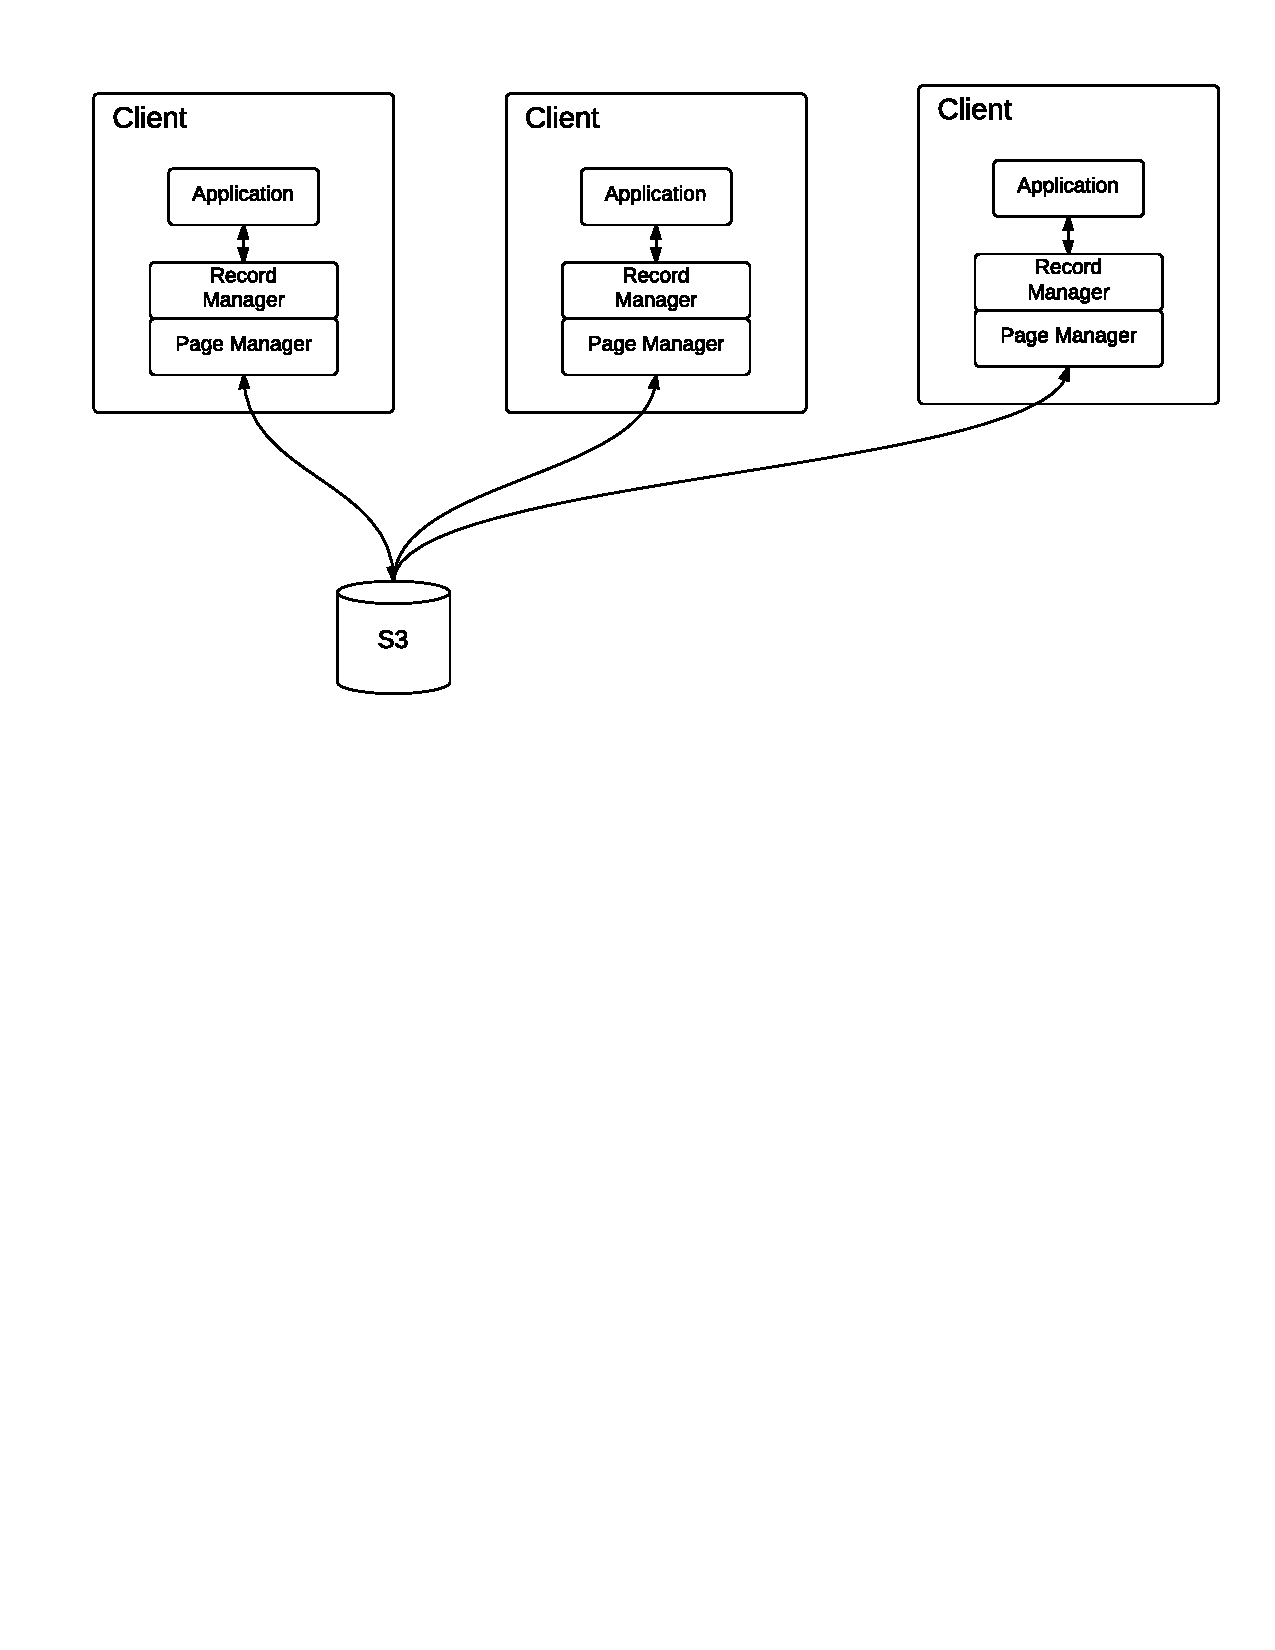
\includegraphics[width=\linewidth]{img/ADB arch 3.pdf}
    \end{center}
  \end{frame}

  \begin{frame}{The proposed implementation (continued)}
    \begin{itemize}
    \item
      SQS can be used to implement a simple commit protocol
    \item
      requires that something actually applies the logs
    \item
      e.g. any node in the system, a watchdog 
    \item
      either way we still end up with eventual consistency
      \begin{itemize}
      \item
        ``all accesses to an item will, eventually, return the last updated value given that no new updates occur''
      \end{itemize}
    \end{itemize}
  \end{frame}

  \begin{frame}{Achievable transactional properties}
    \begin{itemize}
    \item
      Atomicity -- yes! e.g. Atomic Queues
    \item
      Consistency -- at least eventually
      \begin{itemize}
      \item
        Monotonic Reads: commit timestamps on pages
      \item
        Monotonic Writes: update counter on pages
      \item
        Read Yo Writes: automatically if monotonic reads
      \item
        Write follows read: yes, updates are applied to cached pages
      \end{itemize}
    \end{itemize}
  \end{frame}

  \begin{frame}{is it any good?}
    \begin{itemize}
      \item
        ``We have made experiments and as a rule of thumb it can be expected that SQS returns only every tenth relevant message.''
      \item
        It's from 2007. Might want to re-do the experiments.
      \item
        Source code isn't available.
      \end{itemize}
    \end{frame}

\section{the general premise}
  \subsection{what about that?}
  \begin{frame}{the good}
    \begin{itemize}
    \item
      yeah it's pretty good if you want a scalable application
      \begin{itemize}
      \item
        I mean who enjoys having to invest in physical infrastructure?
      \item
        physical stuff requires maintenance
      \item
        pay for what you use
        \begin{itemize}
        \item
          the bill reflects actual usage
        \item
          no initial costs
        \end{itemize}
      \end{itemize}
    \end{itemize}
  \end{frame}
  \begin{frame}{the less good}
    \begin{itemize}
    \item
      pay for what you use
      \begin{itemize}
        \item
        would suck to get ddos'd
        \item
        if income doesn't approximately correlate with usage it could cost you money
      \end{itemize}
    \item
      infinitely scalable database doesn't mean the rest of your application is infinitely scalable
    \end{itemize}
  \end{frame}

\end{document}


